\section{Interrupt}
\begin{itemize}
  \item An interrupt is a Hardware initiated procedure that interrupts whatever program is currently executing.
  \item Useful when interfacing with I/O devices that provide or require data at relatively low data transfer rate.
  \item Teo H/W pins for requesting interrupts: INTR and NMI. \newline
  One H/W pin for acknowledging interrupt requested by INTR : INTA \newline
  S/W interrupts: INT, INT0, INT3 and BOUND \newline
  Two flag bits: IF (Interrupt flag) and TF (Trap flag) \newline
  A special return instruction: IRET (or IRETD in 80386, 486,..)
  \item \textbf{Interrupt vector}: Contains address (Segment, offset) of the interrupt service procedure
  \item \textbf{Interrupt vector Table}: Located in the first 1024 bytes of memory at address 000000H - 0003FFH. It contains 256 different 4-byte interrupt vectors.
\end{itemize}
\begin{figure}[h!]
  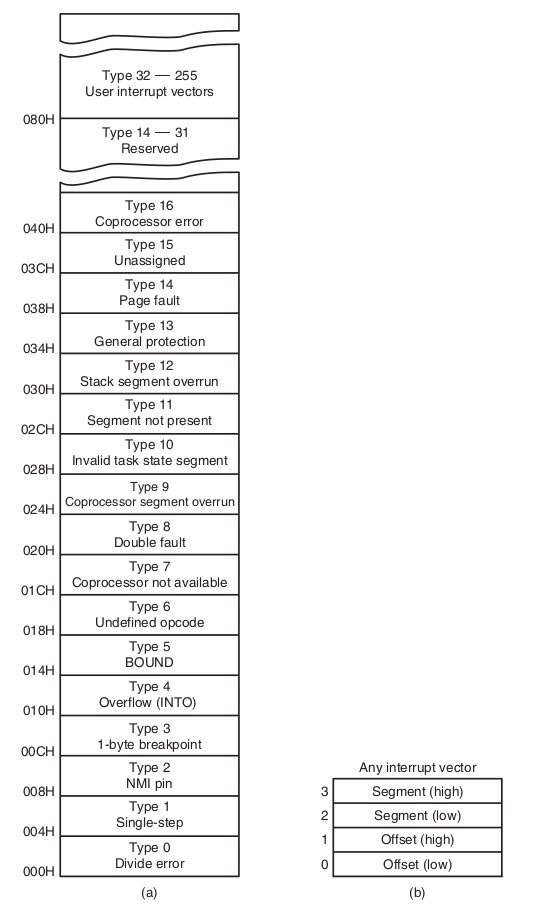
\includegraphics[width = 0.8\textwidth]{./figures/Int_Vect.png}
  \caption{(a) The interrupt vector table for the microprocessor and (b) the contents of an interrupt vector.}
\end{figure}
\begin{itemize}
  \item First 32 interrupt vectors : Reserved
  \item Other 224 interrupt vectors : User defined interrupt vectors
\end{itemize}
Examples of dedicated Interrupts:
\begin{description}
  \item[Type 0] Divide Error$\longrightarrow$ Division overflow oe divide by zero
  \item[Type 1] Single step or Trap $\longrightarrow$ Occurs afterr execution of each instruction. If \textbf{IF} flag is set. Upon accepting this interrupt, IF is cleared to execute interrupt service procedure executes at full speed.
  \item[Type 2] NMI $\longrightarrow$ If 1 is placed in the NMI pin; it annot be disabled
  \item[Type 3] One-Byte Interrupt $\longrightarrow$ INT3; Often used to store a breakpoint in a program for debugging.
  \item[Type 4] Overflow $\longrightarrow$ INT0 ; Interrupts if an overflow condition exists as reflected by Overflow Flag(OF)
  \item[Type 5] Bound $\longrightarrow$ Compares a register with boundary stored in memory. If $1^{st} word in memory \leq reg\leq 2^{nd} word in memory$, no interrupt occurs. Otherwise, an interrupt occurs.
\end{description}
\textbf{INT instruction} : INTn instruction call the interrupt service procedure that begins at the address represented in the vector number n
\begin{itemize}
  \item \textbf{Example}: INT 80H or INT 128 call interrupt service procedure whose address is stored in vector type number 80H(000200H - 000203H)
  \item Each INT instruction is stored in 2 bytes of memory $\longrightarrow$ first byte for opcode, and second byte for interrupt type number.
  \item \textbf{Only exception}: INT3 $\longrightarrow$ 1-byte instruction;  It is 1 byte as it is easy to insert 1-byte instruction ina program for breakpoint.
  \item \textbf{IRET}: Removes six bytes from the stack $\longrightarrow$ 2 for IP , 2 for CS, and 2 for flags
  \item \textbf{Return address of an interrupt}: Next instruction in the program.
  \item \textbf{Return address of BOUND interrupt}: BOUNT instruction itself; \textit{NOT} the next instruction.
  \item \textbf{Similar exception applies for INT type number}: 0,5,6,7,,10,11,12 and 13.

\end{itemize}
Operation of a Real Mode Interrupt :
\begin{enumerate}
  \item Push flag registers in stack
  \item Clear both IF and TF
  \item Push CS (Code Segment Register) in stack
  \item Push IP (Instruction Pointer) in stack
  \item Fetch the interrupt vector contents, and place into both IP and CS so that the next instruction executes at the service procedure addressed by the vector.
\end{enumerate}

\subsection{Operation of a Protected Mode Interrupt}
\begin{itemize}
  \item Uses a set of 25 interrupt descriptors that are stored in any interrupt descriptor table (IDT). The IDT is 256 x  bytes (2KB) long with each descriptor containing  bytes.
  \item The IDT can be located at any place of memory by IDT address register(IDTR)
\end{itemize}

\begin{figure}[h!]
  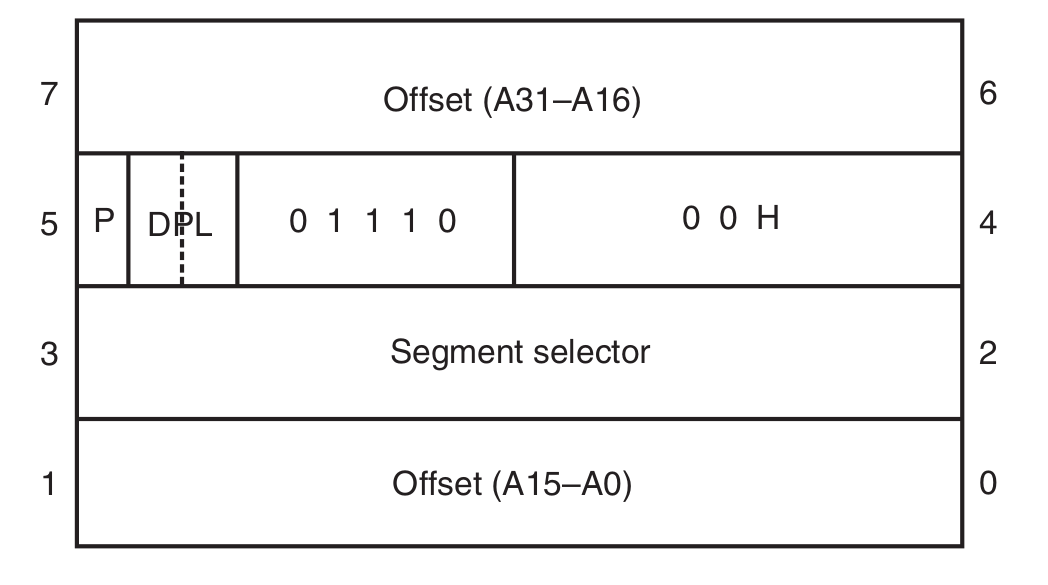
\includegraphics[width = 0.8\textwidth]{./figures/IDT.png}
  \caption{The protected mode interrupt descriptor.}
\end{figure}

\begin{itemize}
  \item \textbf{P bit}: Present
  \item \textbf{DPL bits}: Priviledge level of the interrupt

\end{itemize}
